\section{Experimental design}
We generated queues with process, authentication, and network-flow claims. The generator also recorded whether an observation was original or derived, when it became available, and whether fields were missing or contradictory. Eight training queues and ten development queues informed the method. On the latter, the candidate recalled 169 of 200 expert top-20 incidents, recovered 177, and credited 73 of 100 P@10 positions; it had no false grouped pairs or mixed groups. The planned gate was 170/200 Recall@20, so the candidate missed it by one incident. The team documented a decision to test the candidate unchanged on a new holdout. We report this as a protocol adjustment, not a gate pass.

The new sample used seed 31103 and template variant 2: 15 queues containing 5,018 alerts eligible by the cutoff, or 300 expert top-20 incident opportunities. Both methods received the same alerts. Source and configuration hashes were fixed, and predictions and decision files were SHA-256 sealed before the evaluator opened private truth. We evaluated each arm once. Variant 2 changes the synthetic template, but the holdout still comes from the same generator family. Figure~\ref{fig:protocol} records the order of these steps.
\begin{figure}[ht]\centering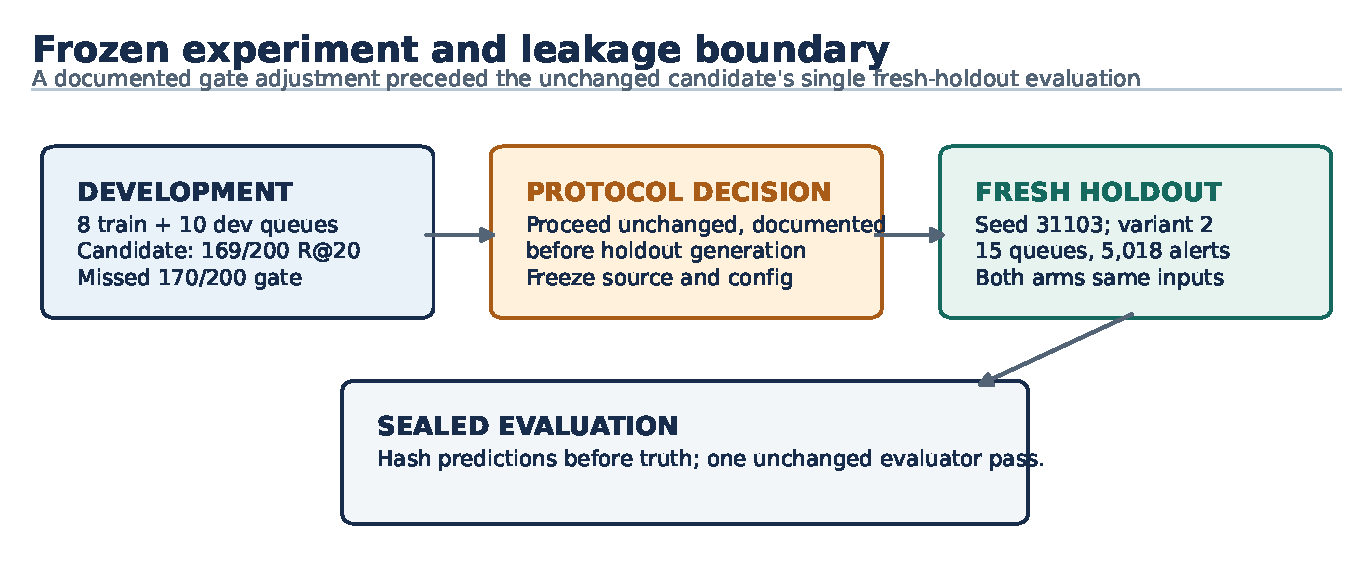
\includegraphics[width=\linewidth]{figures/experimental_protocol.pdf}\caption{Experimental order: training and development, the missed 170/200 development gate, the documented authorization to test the unchanged candidate, a fresh synthetic holdout, SHA-256 sealing, and one subsequent private-truth evaluation. No post-result holdout tuning is represented.}\label{fig:protocol}\end{figure}
\begin{table*}[t]\centering\footnotesize\caption{Distinct research populations. Separate development cohorts in later studies cannot be pooled with the primary holdout.}\label{tab:cohorts}\begin{tabularx}{\textwidth}{@{}p{0.18\textwidth}p{0.21\textwidth}Y@{}}\toprule Population & Size & Role and boundary\\\midrule Controlled training & 8 queues & Generator-family method development; private holdout not involved\\ Controlled development & 10 queues; 200 top-20 opportunities & Candidate selection and one-incident gate miss\\ Frozen holdout & 15 queues; 5,018 eligible alerts; 300 top-20 opportunities & Paired baseline/candidate evaluation after prediction seal\\ Later studies & Separate development cohorts, generally 15 queues each & Diagnostic and ranking investigations; no fresh promoted holdout\\ GUIDE inspection & 4,147,992 evidence rows & Schema/readiness audit; no model predictions\\\bottomrule\end{tabularx}\end{table*}
